\chapter{Implementare Librăriei}

În acest capitol va fii prezentata implementarea librăriei software pentru dezvoltarea de algoritmi și aplicații de recunoaștere a obiectelor.

\section{Diagrama de clase}

Librăria este împărțita în următoarele pachete:
\begin{itemize}
	\item core
	\item dataset
	\item image-pyramid
	\item image-scanning
	\item feature-extraction
	\item classification
	\item non-maxima-suppression
	\item detection
	\item python
\end{itemize}


Pachetul "core" contine interfețe de baza ale librăriei.
\begin{center}
	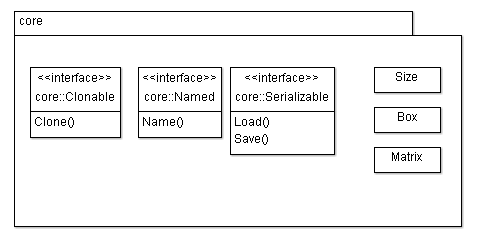
\includegraphics[width=1.00\textwidth]{uml/core_diagram.png}
\end{center}

Pachetul "dataset" contine clase care modelează baza de date pentru antrenament, și implementează funcționalități de importare unor formate uzuale.
\begin{center}
	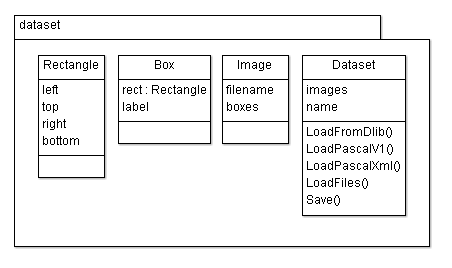
\includegraphics[width=1.00\textwidth]{uml/dataset_diagram.png}
\end{center}

Pachetul "image-pyramid" contine interfețe și implementeri care servesc la construcția piramidei de imagini.
\begin{center}
	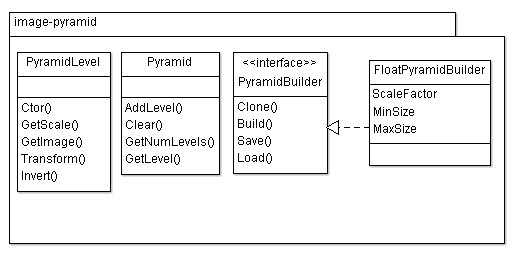
\includegraphics[width=1.00\textwidth]{uml/pyramid_diagram.png}
\end{center}

Pachetul "image-scanning" contine interfete si implementari care servesc la scanarea imaginilor
\begin{center}
	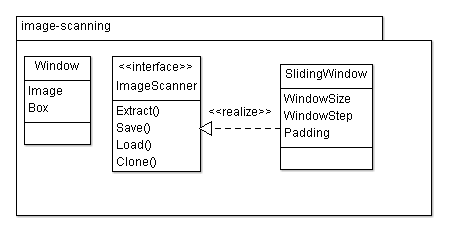
\includegraphics[width=1.00\textwidth]{uml/image_scanning_diagram.png}
\end{center}

Pachetul "feature-extraction" contine interfete si implementari care servesc la extragerea de trasaturi din imagini.
\begin{center}
	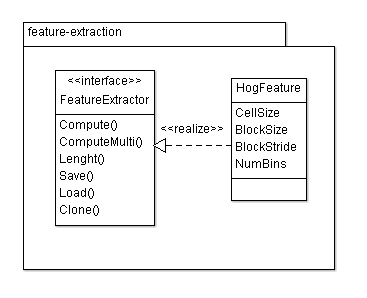
\includegraphics[width=0.8\textwidth]{uml/feature_extraction_diagram.png}
\end{center}

Pachetul "classification" contine interfete si implementari care servesc la clasificare si antrenarea clasificatorilor.
\begin{center}
	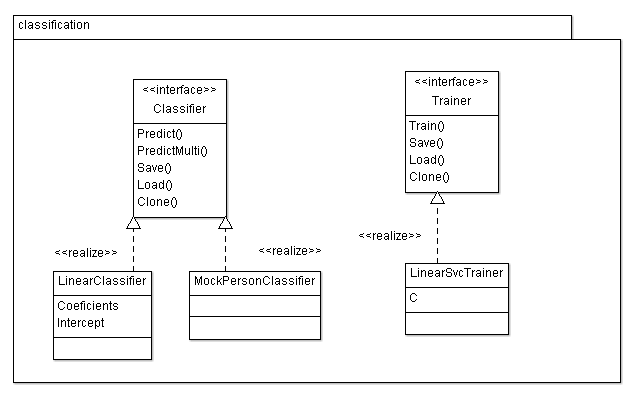
\includegraphics[width=1.00\textwidth]{uml/classification_diagram.png}
\end{center}

Pachetul "non-maxima-suppression" contine interfete si implementari care servesc la post-procesarea rezultatelor.
\begin{center}
	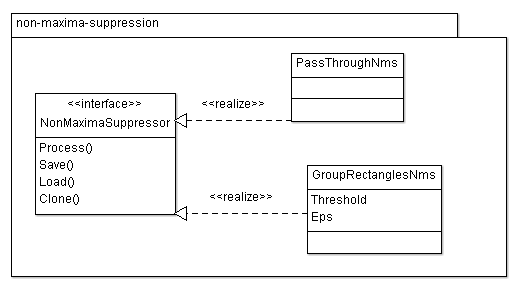
\includegraphics[width=1.00\textwidth]{uml/nms_diagram.png}
\end{center}

Pachetul "detection" contine interfete si implementari care servesc la recunoasterea obiectelor in imagini si la antrenarea algoritmilor.
\begin{center}
	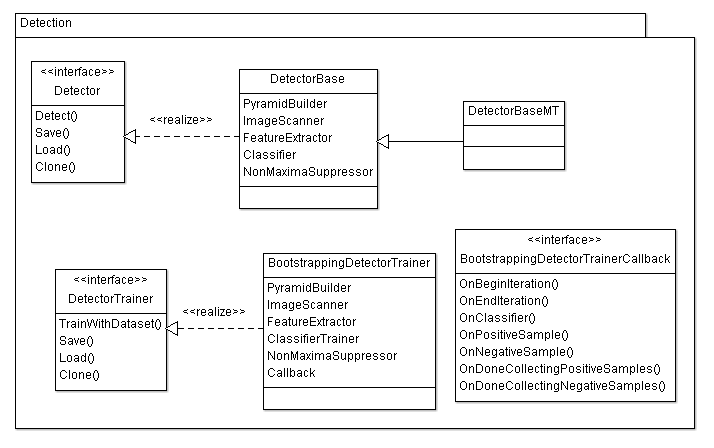
\includegraphics[width=1.00\textwidth]{uml/detection_diagram.png}
\end{center}

Pachetul "python" contine supportul necesar pentru interoperabilitatea cu limbajul Python.



\pagebreak

\section{Interoperabilitatea cu Python}
\pagebreak

\section{Serializarea}
\pagebreak